\documentclass[UTF8, a4paper]{ctexart}

\usepackage{geometry}
\usepackage{titlesec}
\usepackage{titletoc}
\usepackage{graphicx}
\usepackage{caption}
\usepackage{hyperref}

\geometry{a4paper, left = 2.7cm, right = 2.7cm, top = 2.54cm, bottom = 2.54cm}

\captionsetup[figure]{skip=0pt}
\captionsetup[table]{skip=0pt}

\title{基于神经网络回归模型的降雨量问题研究}

\author{李沐阳 \and 易领程 \and 钟绍恒}

\begin {document}

\maketitle

\newpage

\tableofcontents

\addcontentsline{tocloft}{section}{附录}

\newpage

\section{摘要}

本文针对局部地区的降雨量与其它气象相关的因素进行了数学模型的建立和求解的通用算法的设计,运用\textbf{线性回归,障碍计数,时间序列和神经网络}等模型分别进行了尝试,并且使用\textbf{遗传算法}优化了模型的求解。

我们首先针对与降水量关联度最大的\textbf{气压}和\textbf{气温}等条件,将数据按照$30$天为一组进行平均处理整理后,根据气象学上的基本原理,运用线性回归模型拟合真实数据,完成了该简单模型的求解,取得了\textbf{正确率$76 \%$}的良好的预测效果,在这里同时使用了\textbf{最小二乘法}和\textbf{遗传算法}进行拟合,均能够取得很好的效果。在此时还尝试了\textbf{障碍计数模型}来应对未降雨的情况,但尝试后发现准确率极低,只有$10\%$左右,整理数据后分析得到数据的趋势具有连续变量的特征,趋势上大致更加符合回归模型这一类。

随后扩大研究的范围,添加了\textbf{云层覆盖,湿度,风速}为新的自变量,由于此时线性回归在多个自变量的的相互影响下适应性较差,转变模型,根据深度学习的基本原理和神经网络中防止过拟合的技术,运用了神经网络回归模型进行拟合,在仅使用$4$个神经层,共$200$多个神经元的情况下取得了\textbf{绝对平均误差仅为$9mm$}的优异结果 。同时,我们也再次展开了遗传算法的尝试,在仅有$4$层共$10$个神经元的网络中取得了$50\%$的正确率,由于遗传算法在一定程度上的局限无法将神经元数量扩充到太大,但依旧提供了一种解决问题的新思路。

在数据具有明显季节性质,且相邻的日期可能相互影响的情况下,我们也对\textbf{时间序列模型}进行了一定的尝试和研究,最后得到的效果也不如神经网络回归模型,原因可能是相互影响因素已经体现在了自变量中。经过进一步的分析,由于数据间并非存在明显的非线性关系,排除了\textbf{决策树模型}的可能性。尝试和分析过后,最后认为该神经网络模型更加准确。

该模型具有预测率较高,和可以轻易扩展到新的自变量的优点。生成该模型的方法可以轻易地被用于生成\textbf{任何局部降雨模型},非常简单易行。在考虑到气象的周期性而忽略人为影响的情况下,本模型具有较为准确的预测能力。

关键词:\texttt{神经网络回归模型}  \texttt{线性回归模型}  \texttt{遗传算法}

\newpage

\section{问题重述}

\subsection{问题背景}

在过去的几十年中,随着各行各业的迅速发展,气象对于人类生产生活的影响日益显著,对于气象预测的精确程度需要愈来愈高,降雨作为人们出行和农业生产的客观需要是非常关键的一部分。在当今时代,由于人类活动的影响日益增大和气象全球性变化的影响下,气象的预测越来越有必要与时俱进,因地制宜的适应局部气候的变化。


\section{模型假设和符号说明}

该模型假设气象活动完全是周期性的,不考虑气候的逐渐变化,也不考虑人为因素的气候的干扰。

\begin{table}[h]
	\centering
	\caption{符号说明}
	\begin{tabular}{p{6em}l}
		\hline
		符号  & 说明     \\
		\hline
		$r$ & 降雨量    \\
		$y$ & 模型的因变量 \\
		\hline
	\end{tabular}
\end{table}

\section{模型建立与求解}

首先,从附录2中获取关于11号气象站(一个奥地利气象站)中的相关数据,考虑到尽可能减少人类活动的影响,本文主要研究该地区从1877年到1917的局部降水量。首先研究降水量与气压和温度的关系,获取完数据之后,按照$30$天为一组进行平均,画出各个自变量的图像如下
\begin{figure}[h!]
	\centering
	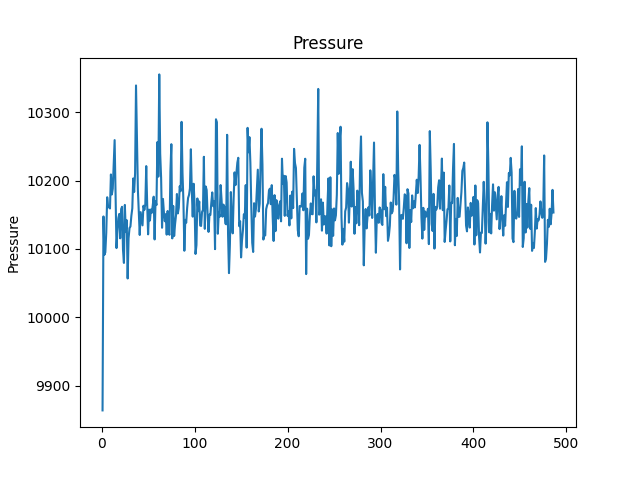
\includegraphics[scale=0.5]{pp.png}
	\caption{气压覆盖关于时间的折线图}
\end{figure}


\begin{figure}[h!]
	\centering
	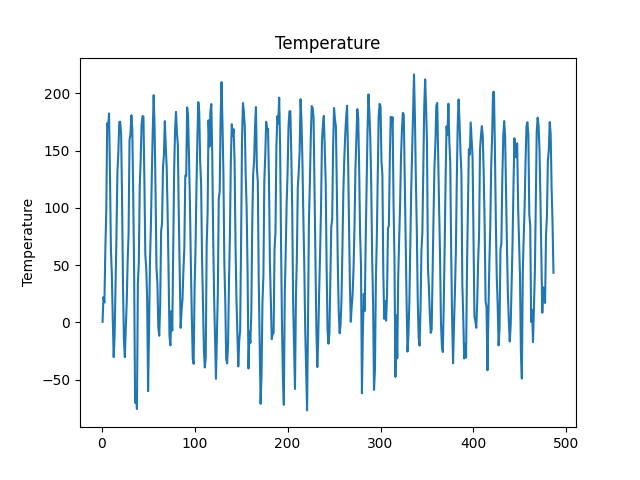
\includegraphics[scale=0.5]{tg.png}
	\caption{气温关于时间的折线图}
\end{figure}

\begin{figure}[h!]
	\centering
	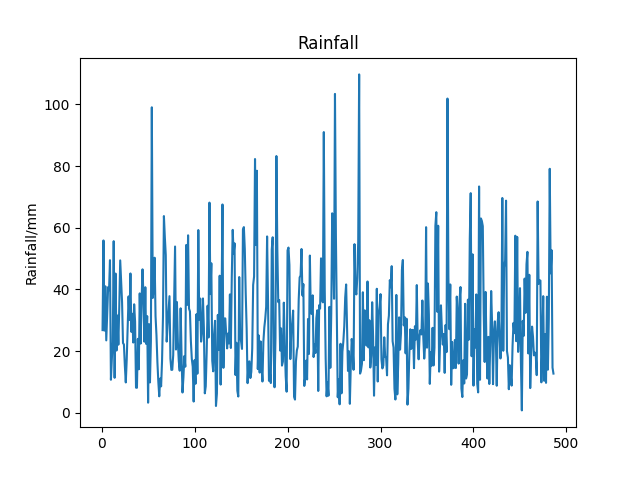
\includegraphics[scale=0.5]{rr.png}
	\caption{降水量关于时间的折线图}
\end{figure}

简单研究,发现这3个量之间很可能呈线性关系,设降雨量为$y$,气压为$a$, 温度为$b$, 建立线性回归模型 $y=pa+qb$,使用最小二乘法让程序生成对应的模型(该程序见附录3),从而拟合最多的数据,得到结果为$y=$,画出拟合图像与真实图像:

\begin{figure}[htbp]
	\centering
	
\includegraphics[scale=0.1]{rust.jpg}
	\caption{拟合降水量和真是降水量的折线统计图}
\end{figure}


\section{模型的优缺点与改进方法}


\section{参考文献}


\appendix
\setcounter{secnumdepth}{-2}
\section{附录}

\setcounter{secnumdepth}{3}
\subsection{源代码}

\subsection{数据来源}

\href{https://www.ecad.eu/}{European Climate Assessment  Dataset}

\end {document}
